\documentclass[aspectratio=169, 12pt]{beamer}

\usepackage[bgphoto]{Configuration_Files/beamerthemepolimi}

% Full instructions available at:
% https://github.com/elauksap/beamerthemepolimi

% Set custom font (requires to compile with XeLaTeX).
\usepackage{ifxetex}
\ifxetex
    \usepackage{fontspec}
    \setsansfont[Scale=0.95]{Arial}
\fi

% STANDARD MATH PACKAGES
\usepackage{amsmath}
\usepackage{amsthm}
\usepackage{bm}
%\usepackage[overload]{empheq}  % For braced-style systems of equations

% REFERENCES PACKAGES
\usepackage[capitalize]{cleveref}

% COLOR
\usepackage{xcolor}

% IMAGES
\usepackage{wrapfig}

\newcommand{\gbm}[1]{\bm{\mathbf{#1}}} % General Bold Math for both greek and latin letters
\newcommand{\rowcolorhang}[1]{\rowcolor{#1}[\dimexpr\tabcolsep+0.1pt\relax]} % Add overang to table row coloring, to avoid vertical white lines
\creflabelformat{equation}{#2\textup{#1}#3} % Remove parentheses from cleveref equations
\newcommand{\T}{\mathrm{T}} % Transpose

\title{Interpreting Large Language Models Through the Lens of Embedding-Oriented Visualizations: Markov Models, Sankey Diagrams and Comparative Approaches}
%\subtitle{}
\author{Davide Rigamonti}
\advisor{Prof. Mark Carman}
\coadvisors{Nicolò Brunello, Vincenzo Scotti}
\date{03/04/2025}

\begin{document}

    \begin{frame}
        \maketitle
        % If the theme option "nologo" is specified, a custom logo
        % can be added with the following commands:
        %\begin{tikzpicture}[overlay, remember picture]
        %    \node at (current page.north) [anchor=north, inner sep=2cm]
        %    {
        %        
\includegraphics[width=0.3\paperwidth]{logo_centrato_BN_negativo.png}
        %    };
        %\end{tikzpicture}
    \end{frame}
    
    \begin{frame}{Table of Contents}
      \tableofcontents
    \end{frame}
    
    \section{Introduction}

    \begin{frame}{}
        \textcolor{red}{TODO}
    \end{frame}

    \begin{frame}{}
        \begin{itemize}[<+|visible@+->]
            \item \textbf{Question:} How can we visualize internal states of LLMs in an immediate and interactive way?
            \item \textbf{Proposed Solution:} Development of an interactive visualization tool for LLMs, \emph{InTraVisTo (Inside Transformer Visualization Tool)}, designed to support machine learning researchers in hypothesis formulation by offering a unique perspective on the internal representations of LLMs.
        \end{itemize}
    \end{frame}

    \begin{frame}{}
        \begin{itemize}[<+|visible@+->]
            \item<1-1> \textbf{Question:} Do autoregressive LLMs retain linear properties in their embedding spaces?
            \item<2-4> \textbf{Proposed Solution:} Use experiments based on analogies to assess the relationship between distance and semantic/morphological similarity on the embedding spaces of recent models.
            \begin{itemize}[<+|visible@+->]
                \item<3-3> Identify key differences in the embedding spaces generated by classic transformer architectures against autoregressive LLMs.
                \item<4-4> Clarify how the shift from the input representation to the output one affects the embedding spaces involved through the layers of an LLM.
            \end{itemize}
        \end{itemize}
    \end{frame}

    \begin{frame}{}
        \begin{itemize}[<+|visible@+->]
            \item<1-1> \textbf{Question:} Is it possible to obtain first-order predictions by concatenating embedding spaces in LLMs?
            \item<2-4> \textbf{Proposed Solution:} Compare a trained bigram Markov model and an identity matrix against the transition matrix of a First Order Model (FOM) obtained by multiplying the embedding and unembedding matrices of an LLM.
            \begin{itemize}[<+|visible@+->]
                \item<3-3> Evaluate similarity or dissimilarity between the transition matrices using direct matrix comparison and set similarity metrics.
                \item<4-4> Evaluate similarity or dissimilarity between the transition matrices using probabilistic metrics such as perplexity and KL divergence.
            \end{itemize}
        \end{itemize}
    \end{frame}

    \begin{frame}{}
        \center
        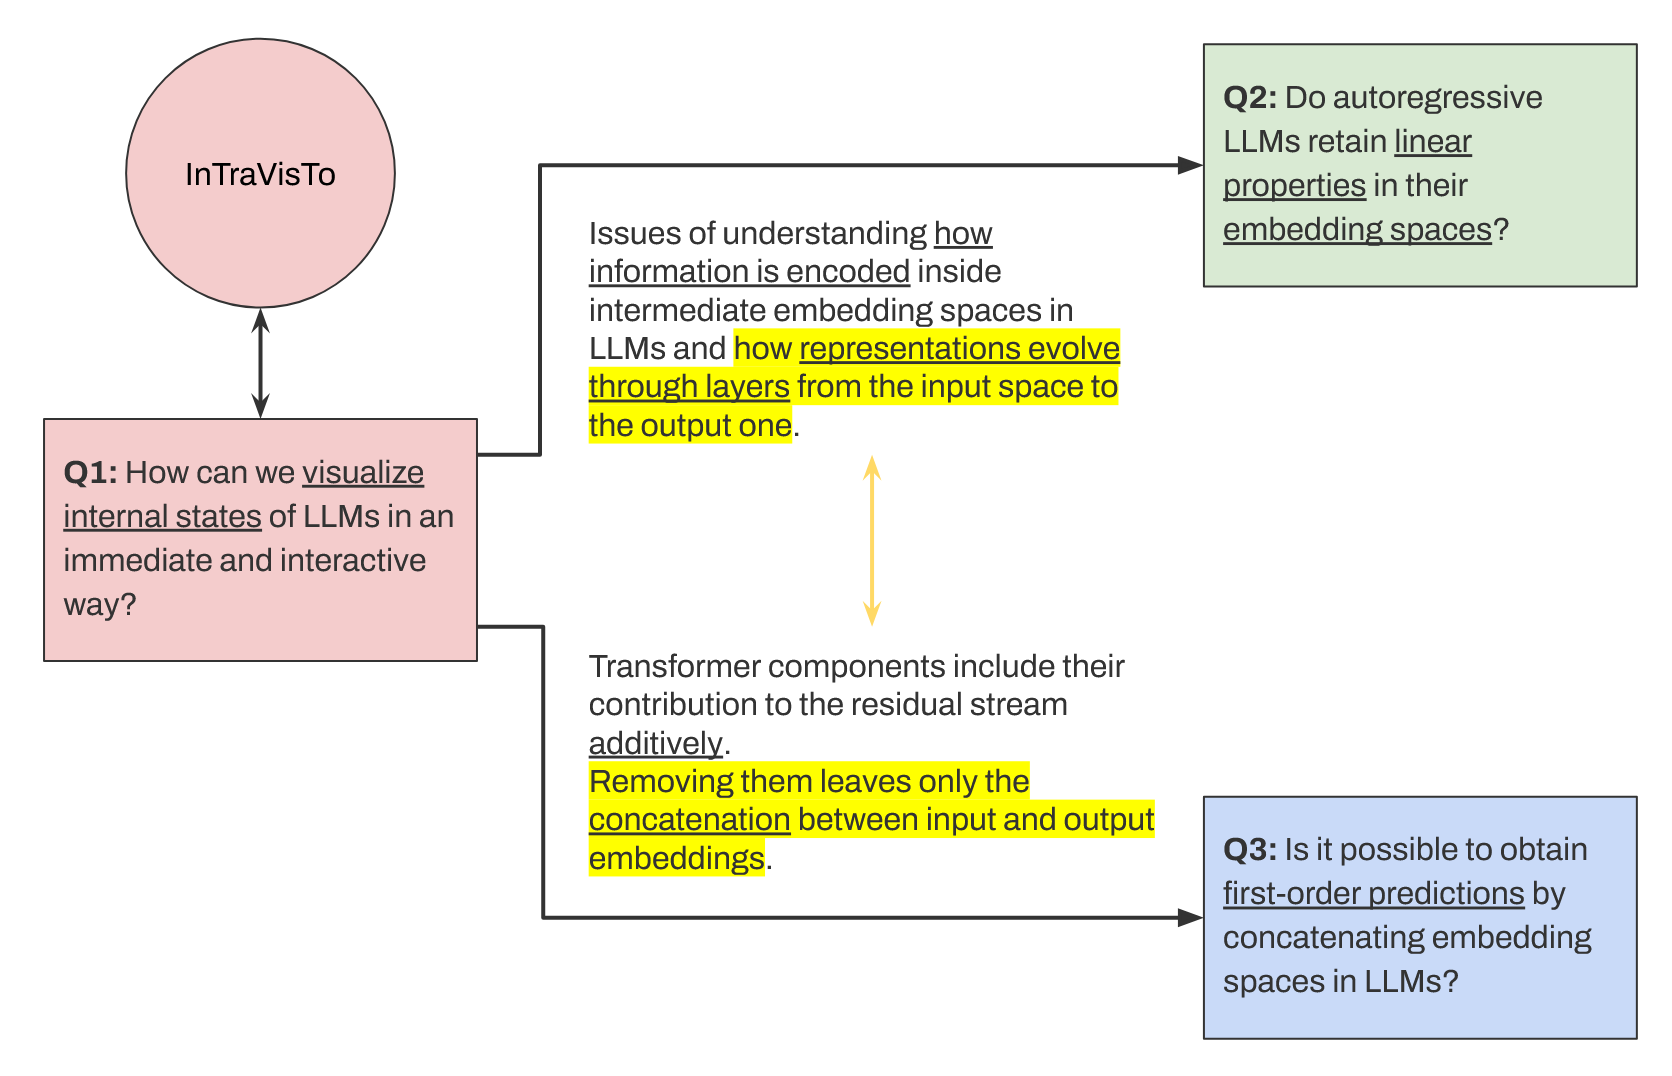
\includegraphics[width=0.6\textwidth]{thesis-flow.png}
    \end{frame}

    \section{State of the Art}

    \begin{frame}{}
        \textcolor{red}{TODO}
        One of the most direct methods to comprehend a model's hidden representations is by employing its own vocabulary to derive plausible interpretations.
        \textbf{Vocabulary space decoding} techniques are founded on this principle, by utilizing the model's existing vocabulary they can generate outputs that are immediately understandable and may unveil hidden patterns inside the model's generation process.
    \end{frame}

    \begin{frame}{}
        \textcolor{red}{TODO}
        A more recent iteration of the vocabulary space decoding approach is the \emph{LM Transparency Tool (LM-TT)}, which is an exceptional toolkit offering interactive tools for analyzing the internal workings of Transformer models.
        LM-TT builds on top of the circuital interpretation of the Transformer to visualize the information flow.
        The LM-TT tool focuses on the visualization of the most relevant attention paths leading to the production of an embedding in the internal states of the Transformer.
        Additionally, it also provides useful decoding information that can aid the interpretation of intermediate representations at varying degrees of granularity.
    \end{frame}

    \section{Transformer Visualization}

    \subsection{Methodology}

    \begin{frame}{}
        \textcolor{red}{TODO}
        InTraVisTo allows decoding and inspection of the \emph{main four vectors} that compose each layer, while offering a human-interpretable representation of each hidden state by performing a decoding operation.
        The four vectors correspond respectively to the output of the attention component, the intermediate state given by the addition of the attention component to the residual stream, the output of the feed-forward network component, and the layer output.
        On the other hand, the decoding operation is carried out using a specialized decoder which, given a hidden state as input, finds related tokens from the model's vocabulary with the goal of returning an interpretable output.
    \end{frame}

    \subsubsection{Decoding Interface}
    \begin{frame}{}
        Decoding the meaning of hidden state vectors at various depths of a Transformer stack is essential for providing an intuition as to how the model is working.

        \begin{equation*}
        \begin{gathered}
            \uncover<+|visible@1+->{
                P(\ \cdot \mid \gbm{x}, d_{\textit{dec}}, n_{\textit{norm}}) = P(\ \cdot \mid \gbm{x}, \gbm{W}_{d_{\textit{dec}}}, N_{n_{\textit{norm}}}) = \operatorname{softmax}\Bigl(N_{n_{\textit{norm}}}(\gbm{x}) \cdot \gbm{W}_{d_{\textit{dec}}}\Bigr)
            }\\[15pt]
            %
            \uncover<+|visible@2+->{
                N_{n_{\textit{norm}}}(\gbm{x}) = 
                \left\{
                \begin{array}{cl}
                    \gbm{x} &\ \text{if}\ n_{\textit{norm}} = \text{`no normalization'} \\
                    \mathcal{N}{(\gbm{x})} &\ \text{if}\ n_{\textit{norm}} = \text{`normalize only'} \\
                    \gbm{\gamma} \odot \mathcal{N}{(\gbm{x})} + \gbm{\beta} &\ \text{if}\ n_{\textit{norm}} = \text{`normalize and scale'}
                \end{array}
                \right.
            }\\[15pt]
            %
            \uncover<+|visible@3+->{
                d_{\textit{dec}} \in \bigl\{\text{`input'}, \text{`output'}, \text{`linear'}, \text{`quadratic'}, \text{`max-prob'} \bigr\}
            }\\
        \end{gathered}
        \end{equation*}
    \end{frame}

    \begin{frame}{}
        \begin{itemize}
            \item Natural choices for decoders are the transpose of the \emph{input embedding matrix} $\gbm{W}_{\textit{in}}^\T$, and the \emph{output unembedding matrix} $\gbm{W}_{\textit{out}}$.
            \item InTraVisTo also offers the possibility of decoding hidden states by \emph{interpolating} the input and output decoders based on the layer depth $\ell\in\{0,\ldots,L\}$:
        \end{itemize}
        \begin{equation*}
        \begin{aligned}
                \gbm{W}_{\textit{linear}}^{(\ell)} &=\left(1-\frac{\ell}{L}\right) \cdot \gbm{W}_{\textit{in}}^\T + \frac{\ell}{L} \cdot \gbm{W}_{\textit{out}} \\
                \gbm{W}_{\textit{quadratic}}^{(\ell)} &=\left(1-\left(\frac{\ell}{L}\right)^2\right) \cdot \gbm{W}_{\textit{in}}^\T + \left(\frac{\ell}{L}\right)^2 \cdot \gbm{W}_{\textit{out}} \\
                \gbm{W}_{\textit{max\_p}} &=\operatornamewithlimits{argmax}_{\gbm{W} \in \{\gbm{W}_{\textit{in}}^\T, \gbm{W}_{\textit{out}}\}} \operatornamewithlimits{max}_{v \in \mathcal{V}} P(v \mid \gbm{x}, \gbm{W}, N_{n_{\textit{norm}}}) \\
        \end{aligned}
        \end{equation*}
    \end{frame}

    \begin{frame}{}
        \begin{minipage}{0.45\textwidth}
            \begin{itemize}
                \item Each cell represents a token-layer combination contained the main decoded hidden state in token form.
                \item By hovering on a cell, a pop-up with other possible decoded tokens (secondary representation) along with additional information appears.
                \item The generation of the heatmap requires the user to choose a \emph{target embedding}, a \emph{decoding strategy} and a \emph{probability} to display.
            \end{itemize}
        \end{minipage}%
        \begin{minipage}{0.55\textwidth}
            \centering
            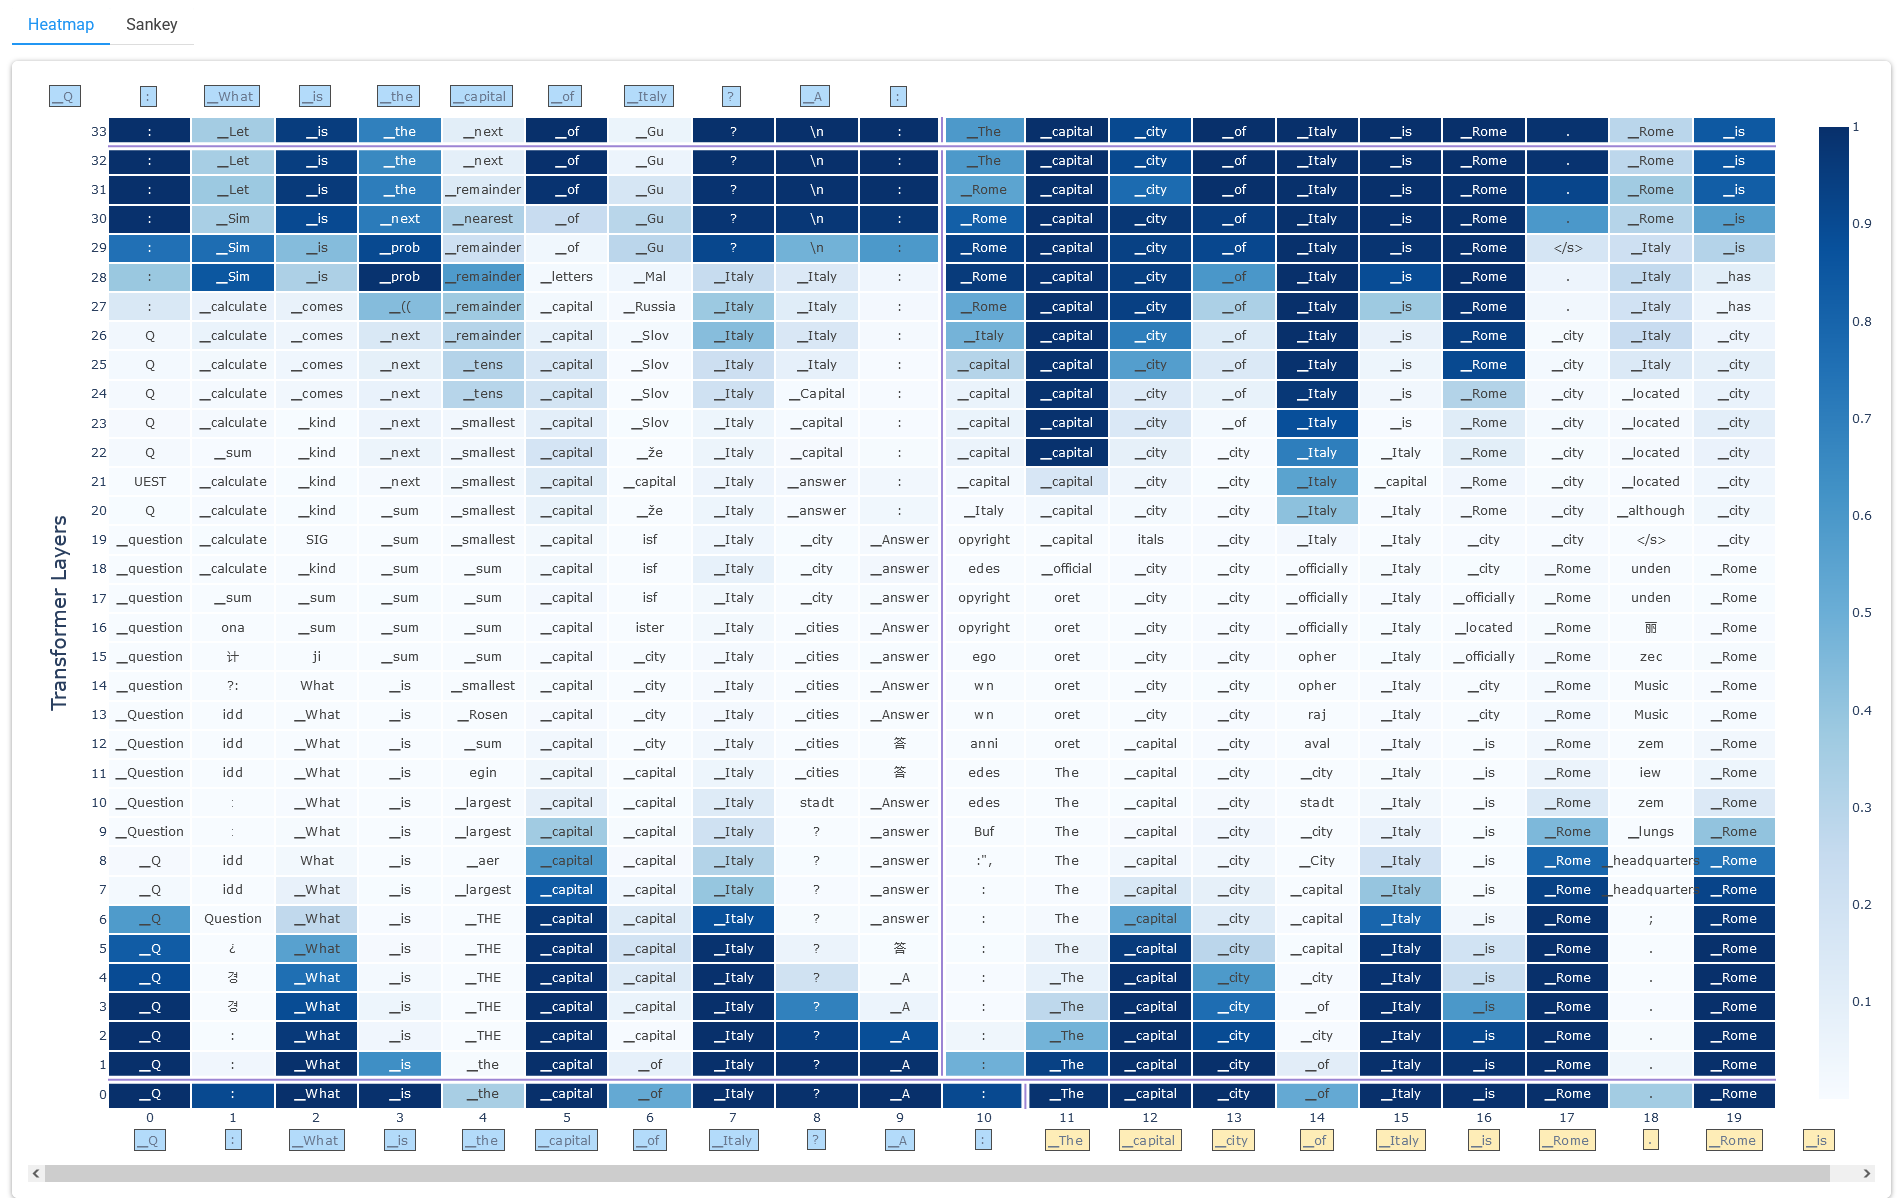
\includegraphics[width=\textwidth]{exp_intravisto_1A_heatmap.png}
        \end{minipage}
    \end{frame}

    \subsubsection{Flow Interface}
    \begin{frame}{}
        \begin{minipage}{0.59\textwidth}
            \begin{itemize}
                \item The second visualization provided by InTraVisTo is a \emph{Sankey diagram} that aims to depict the information flow through the Transformer network.
                \item Nodes in the diagram depict all hidden states contained in each layer, visualizing the four vectors at the same time.
                \item Edges represent the amount of relevance carried by the residual stream, showing how components accumulate or disperse this flow.
            \end{itemize}
        \end{minipage}%
        \begin{minipage}{0.41\textwidth}
            \centering
            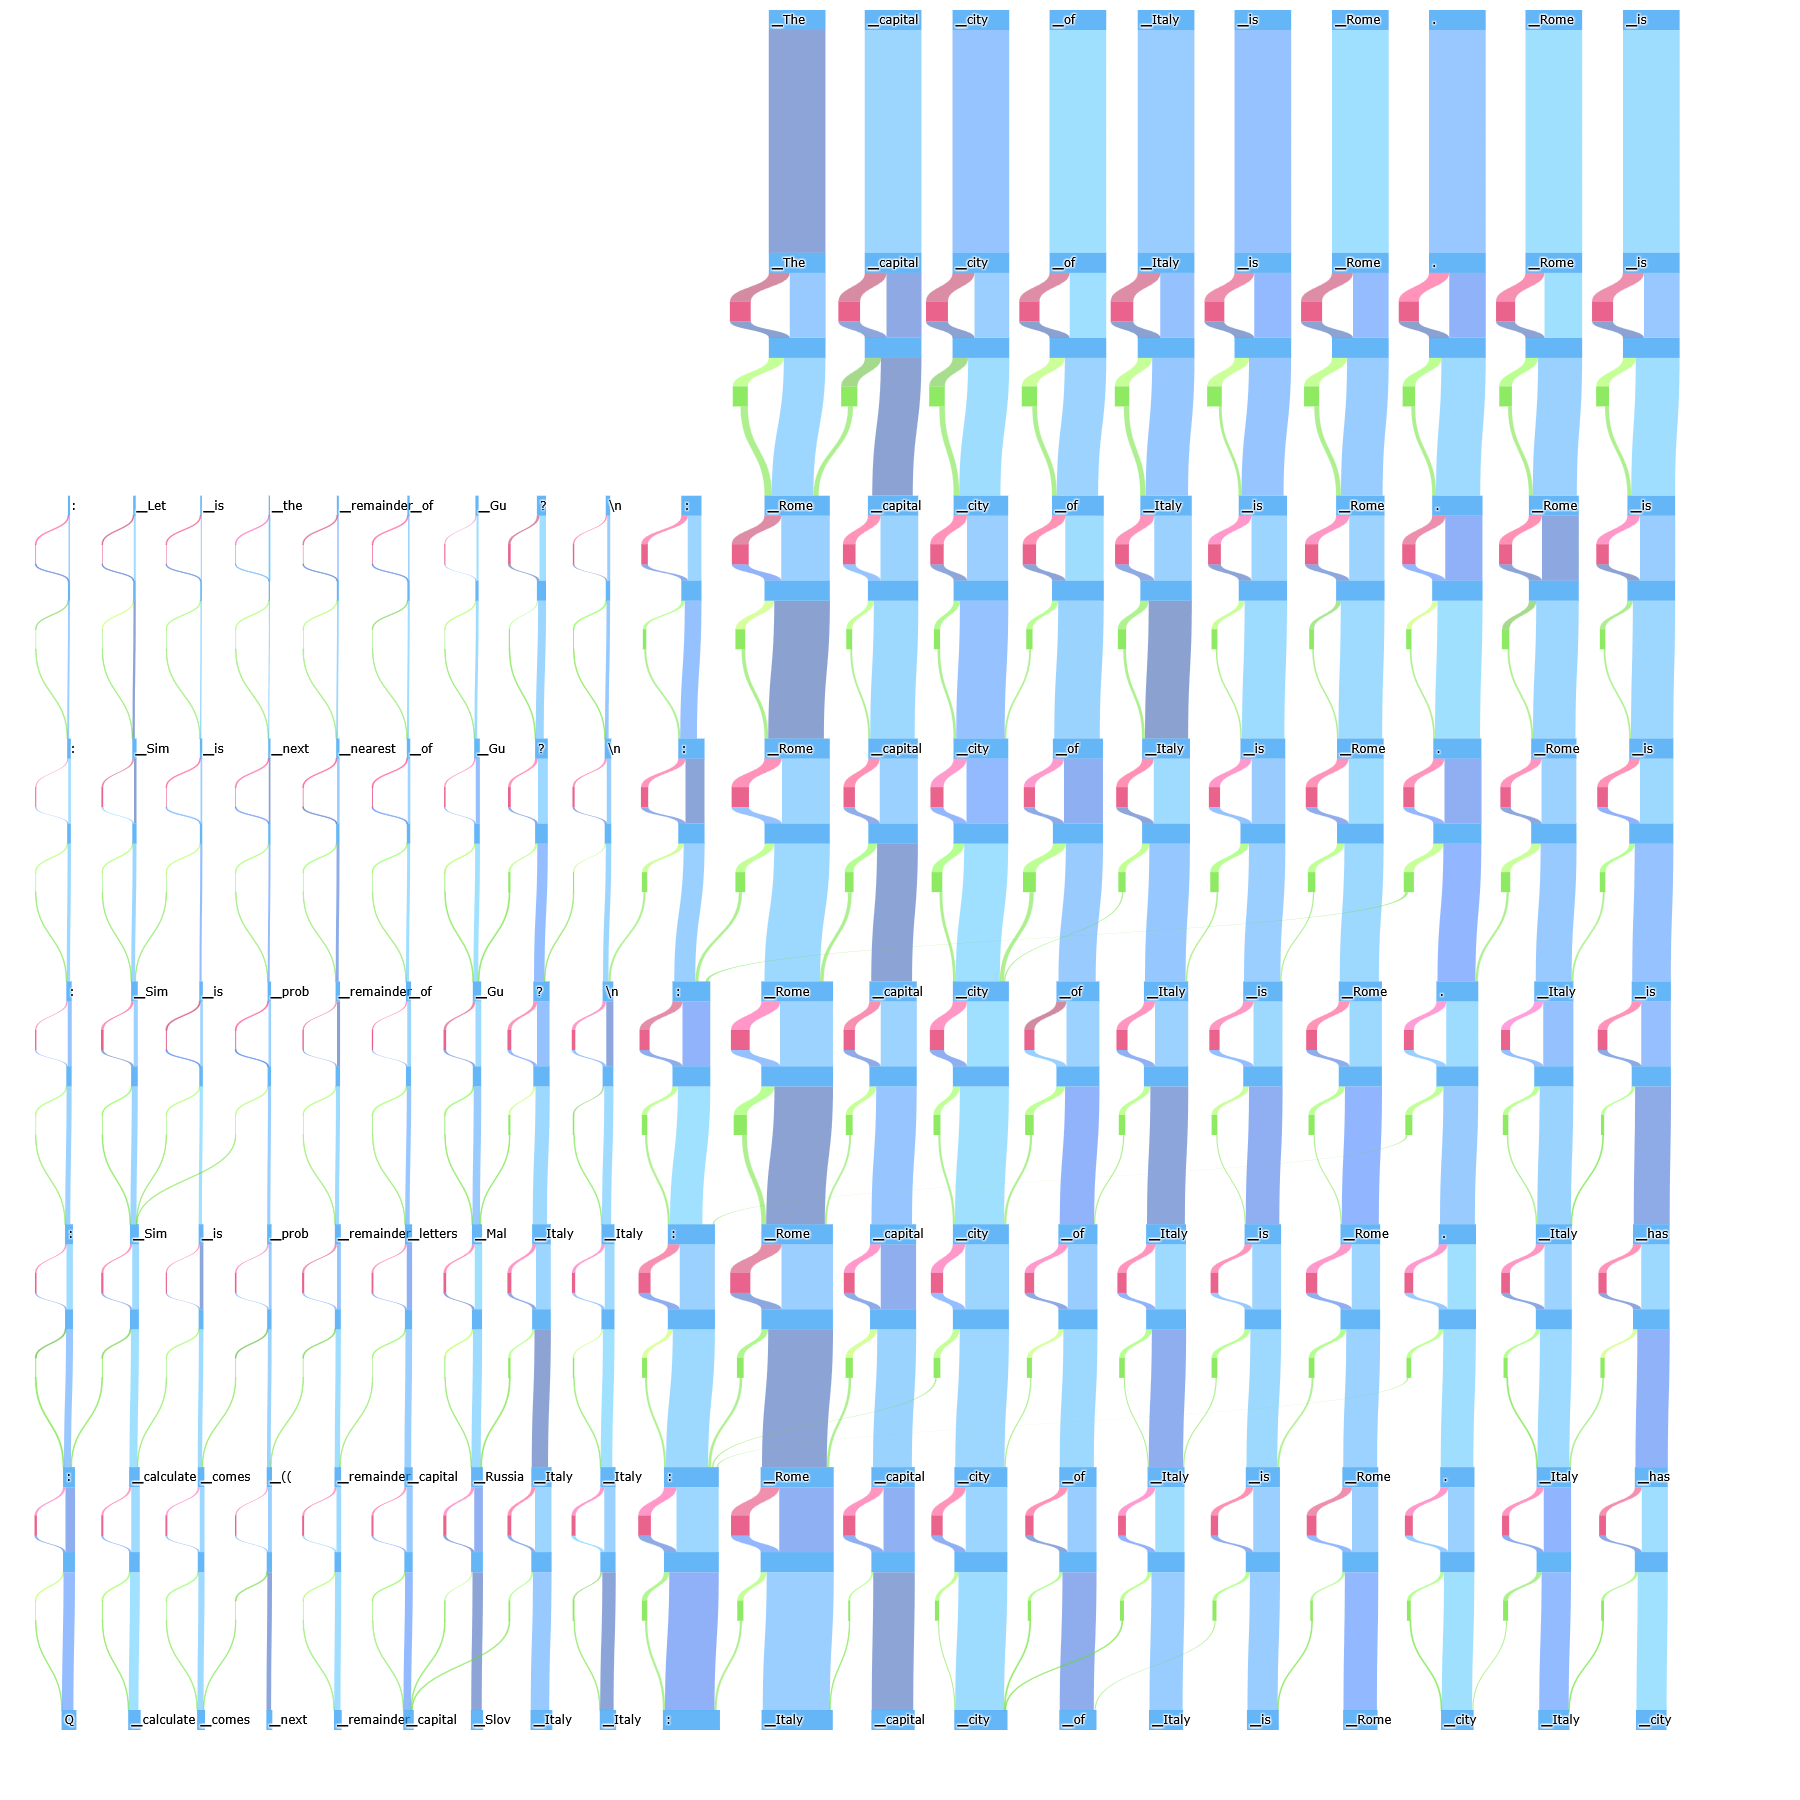
\includegraphics[width=\textwidth]{exp_intravisto_2A_sankey.png}
        \end{minipage}
    \end{frame}

    \begin{frame}{}
        The flow originates from the topmost layer of nodes, equally split between them, and is recursively computed considering the contributions of each encountered node.

        \begin{equation*}
            \left\{
            \begin{alignedat}{2}
                &\textit{flow}_{\textit{ffnn}}^{(\ell,j)} &&= {\%}_{\textit{ffnn}}^{(\ell,j)} \cdot \textit{flow}_{x}^{(\ell,j)} \\
                &\textit{flow}_{x'}^{(\ell,j)} &&= \textit{flow}_{\textit{ffnn}}^{(\ell,j)} + (1 - {\%}_{\textit{ffnn}}^{(\ell,j)}) \cdot \textit{flow}_{\textit{x}}^{(\ell,j)} = \textit{flow}_{\textit{x}}^{(\ell,j)} \\
                &\textit{flow}_{\textit{att}}^{(\ell,j)} &&= {\%}_{\textit{att}}^{(\ell,j)} \cdot \textit{flow}_{x'}^{(\ell,j)} = {\%}_{\textit{att}}^{(\ell,j)} \cdot \textit{flow}_{x}^{(\ell,j)} \\
                &\textit{flow}_{x}^{(\ell-1,j)} &&= \sum_{i\in\{j,\ldots,k\}}{\overline{\textit{attend}{\,}}^{(\ell,i)}\bigl[j\bigr]}\cdot\textit{flow}_{\textit{att}}^{(\ell,i)} + ( 1 - {\%}_{\textit{att}}^{(\ell,j)})\cdot \textit{flow}_{\textit{x'}}^{(\ell,j)} \\
                    &\quad &&= \biggl(\Bigl(\sum_{i\in\{j,\ldots,k\}}\overline{\textit{attend}{\,}}^{(\ell,i)}\bigl[j\bigr] - 1\Bigr)\cdot{\%}_{\textit{att}}^{(\ell,j)} + 1\biggr) \cdot \textit{flow}_{\textit{x}}^{(\ell,j)}
            \end{alignedat}
            \right.
        \end{equation*}
    \end{frame}

    \begin{frame}{}
        \textcolor{red}{TODO}
        \begin{itemize}
            \item Nodes display the main decoding result as their label and, when hovered upon, show additional information in the form of a pop-up tooltip containing secondary representations.
            \item Output nodes' tooltips also include the \emph{decoded difference from the previous layer}, obtained between the current and previous output states with the goal of trying to visualize in a human interpretable way the information added by the current layer relative to the previous one.
            \item If the user inspects a specific cell in the heatmap by clicking on it, the Sankey diagram adapts by recalculating the flow considering the clicked node as the sole topmost node, consequently accounting for $100\%$ of the flow.
        \end{itemize}
    \end{frame}

    \subsubsection{Dinamically Changing the Network}
    \begin{frame}{}
        \begin{minipage}{0.82\textwidth}
        \begin{itemize}
            \item Injections are performed by clicking on a cell in the heatmap or Sankey diagram and substitute hidden states with custom embedding representations, forcing the model to adjust its behavior based on the injected information.
            \item Once a valid injection is compiled and added, a small card summarizing the injection appears at the top of the interface.
            \item If the chosen node corresponds to a feed-forward or an attention node, there is an additional option that allows the user to remove the node, performing an \emph{ablation}.
        \end{itemize}
        \end{minipage}%
        \begin{minipage}{0.18\textwidth}
            \centering
            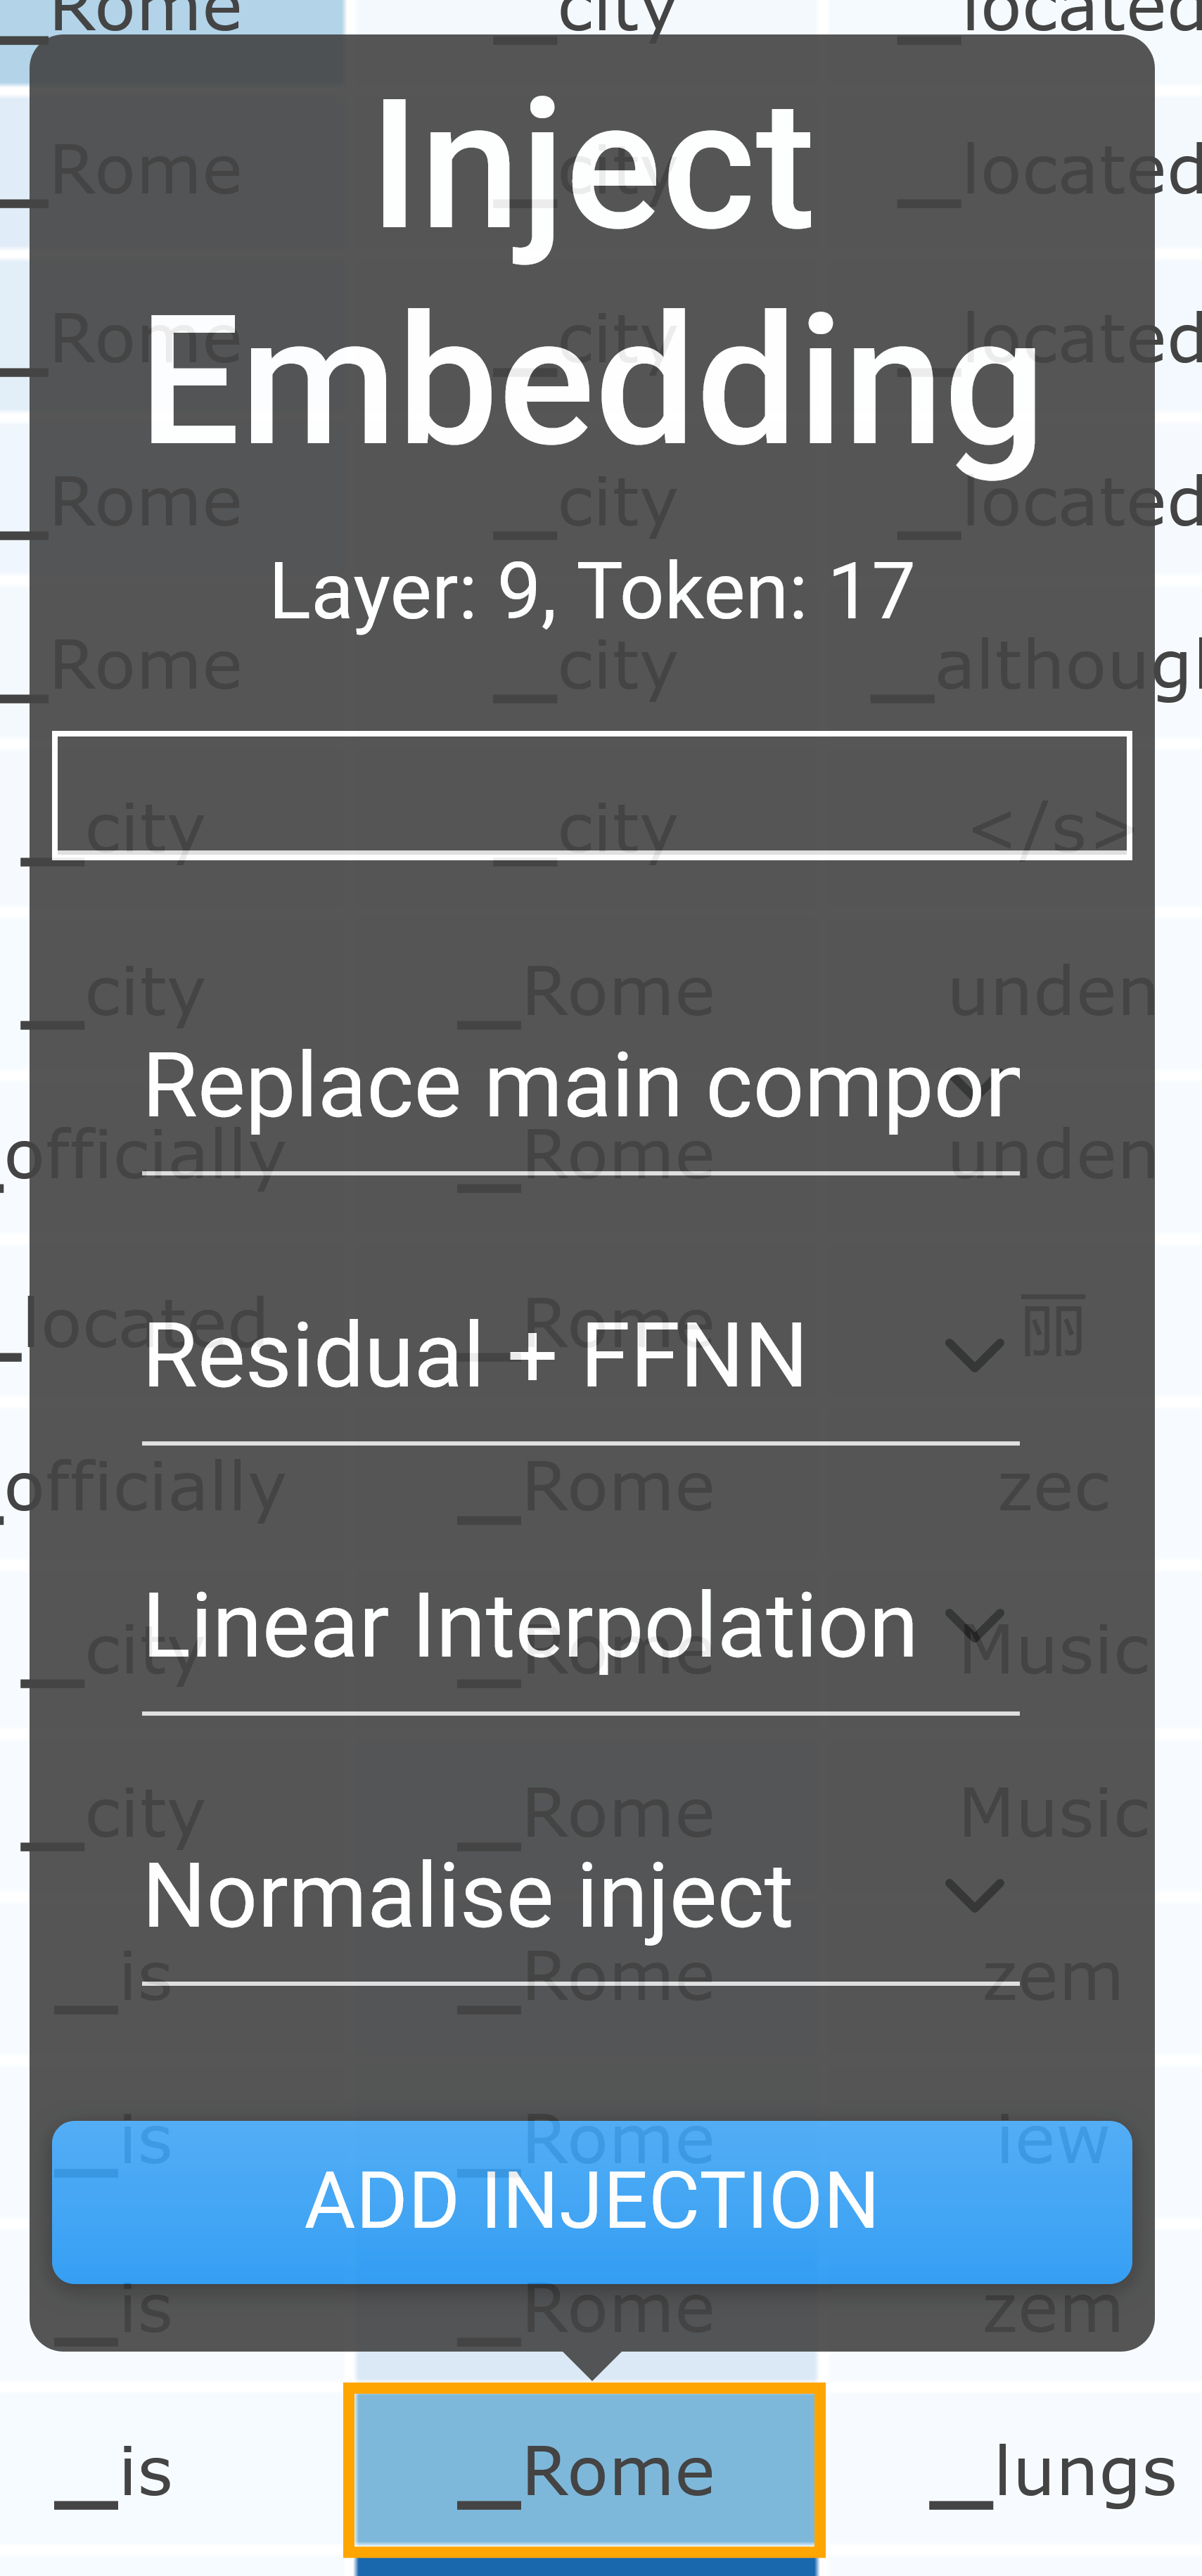
\includegraphics[width=\textwidth]{exp_intravisto_3A_popup.png}
        \end{minipage}
    \end{frame}

    \subsection{Results}
    \begin{frame}{}
        \textcolor{red}{TODO}
    \end{frame}

    \section{Embedding Analysis}

    \subsection{Methodology}
    \begin{frame}{}
        Solving word analogies showcases an embedding space's ability to model word semantics in a relatively consistent way, implying the existence of embedding dimensions with associated meanings (even if overlapping or under superposition).
        \begin{equation*}
            \begin{gathered}
                closest = \operatornamewithlimits{argmin}_{v \in \mathcal{V}} d_{\textit{dist}}\bigl(\tilde w, \textit{encode}^{\textit{emb}}(v)\bigr) \\[15pt]
                \textit{acc}_k = \frac{1}{n} \sum_{i=1}^{n} \mathbb{I}\Bigl( {\left\{ {\textit{result}\,}^i_j \ |\ \forall j = 1,\ldots,k \right\}} \cap {\textit{sol}\,}^i \neq \emptyset \Bigr)
            \end{gathered}
        \end{equation*}
    \end{frame}

    \begin{frame}{}
        \begin{equation*}
            \begin{gathered}
                \begin{aligned}
                    \tilde w &= \textit{analogy}(w_1, w_2, w_3, w_4) \color{gray} \approx {\textit{encode}}_{\textit{enc\_strat}}^{out}(w_3) \\[5pt]
                    &= {\textit{encode}}_{\textit{enc\_strat}}^{in}(w_1) - {\textit{encode}}_{\textit{enc\_strat}}^{in}(w_2) + {\textit{encode}}_{\textit{enc\_strat}}^{in}(w_4)
                \end{aligned} \\[15pt]
                \begin{aligned}
                    {\textit{encode}}_{\textit{enc\_strat}}^{in}(w) &= 
                    \left\{
                    \begin{array}{cl}
                        \gbm{e}_1^w &\ \text{if}\ \textit{enc\_strat} = \text{`first\_only'} \\
                        \frac{1}{t}\sum_{i=1}^{t}{\gbm{e}_i^w} &\ \text{if}\ \textit{enc\_strat} = \text{`average'} \\
                        \sum_{i=1}^{t}{\gbm{e}_i^w} &\ \text{if}\ \textit{enc\_strat} = \text{`sum'}
                    \end{array}
                    \right. \\[10pt]
                    {\textit{encode}}_{\textit{enc\_strat}}^{out}(w) &= 
                    \left\{
                    \begin{array}{cl}
                        \{ tok_1^w \} &\ \text{if}\ \textit{enc\_strat} = \text{`first\_only'} \\
                        \{ tok_1^w, \ldots, tok_t^w \} &\ \text{if}\ \textit{enc\_strat} = \text{`subdivide'}
                    \end{array}
                    \right.
                \end{aligned}
            \end{gathered}
        \end{equation*}
    \end{frame}

    \subsection{Results}
    \begin{frame}{}
        \textcolor{red}{TODO}
    \end{frame}

    \section{First Order Prediction}

    \subsection{Methodology}
    \begin{frame}{}
        A \emph{First Order Model (FOM)} is derived by removing all intermediate architectural components from an LLM, retaining only the input and output embedding layers along with the residual connections joining them.
        \begin{equation*}
            \gbm{Q}_{\textit{FOM}} = \operatorname{softmax}(\gbm{Q}_{\textit{FOM}}^{log}) = \operatorname{softmax}(\gbm{W}_{in} \cdot \gbm{W}_{out}^\T)
        \end{equation*}
        We also explore an alternative (FOM with RMS) that incorporates a single \emph{RMS normalization} step between the standard FOM embeddings.
        \begin{equation*}
            \text{where}\ \left\{
                \begin{array}{cl}
                    \gbm{W}_{in,RMS} &= \left(\frac{\gbm{w}_i^{in}}{RMS(\gbm{w}_i^{in})}\right)_{i,\cdot} = \left(\frac{\gbm{w}_i^{in}}{\sqrt{\frac{1}{D}\sum_{j=1}^{D}{(w_{ij}^{in})^2}}}\right)_{i,\cdot} \\
                    \gbm{W}_{out,RMS} &= \left(\gbm{\gamma}^\T \odot \gbm{w}_j^{out}\right)_{\cdot,j}
                \end{array}
            \right.
        \end{equation*}
    \end{frame}

    %\begin{gathered}
    %    \gbm{Q}_{\textit{FOM}}^{RMS} = \operatorname{softmax}(\gbm{W}_{in,RMS} \cdot \gbm{W}_{out,RMS}^\T) \\
    %    \text{where}\ \left\{
    %        \begin{array}{cl}
    %            \gbm{W}_{in,RMS} &= \left(\frac{\gbm{w}_i^{in}}{RMS(\gbm{w}_i^{in})}\right)_{i,\cdot} = \left(\frac{\gbm{w}_i^{in}}{\sqrt{\frac{1}{D}\sum_{j=1}^{D}{(w_{ij}^{in})^2}}}\right)_{i,\cdot} \\
    %            \gbm{W}_{out,RMS} &= \left(\gbm{\gamma}^\T \odot \gbm{w}_j^{out}\right)_{\cdot,j}
    %        \end{array}
    %    \right.
    %\end{gathered}

    \begin{frame}[plain]{}
        \vspace{0.3cm}
        We start by performing a \emph{naïve direct comparison} between transition matrices:
        \begin{equation*}
            \left\{
                \begin{array}{cl}
                    d_{\textit{FOM},I} &= \| \gbm{Q}_{\textit{FOM}} - \gbm{I}_V \|_F \\
                    d_{\textit{FOM},\textit{markov}} &= \| \gbm{Q}_{\textit{FOM}} - \gbm{Q}_{\textit{markov}} \|_F
                \end{array}
            \right.
        \end{equation*}
        Followed by the use of \emph{set similarity metrics} (such as top-$k$ accuracy, Jaccard similarity and overlap coefficient) to obtain more reliable estimates:
        \begin{equation*}
            \begin{gathered}
                \textit{accuracy}_{k_1,k_2}(\gbm{Q}_1, \gbm{Q}_2) = \frac{1}{V} \sum_{v \in \mathcal{V}}{\textit{tok\_overlap}_{k_1,k_2}(\gbm{Q}_1, \gbm{Q}_2, v)} \\
                \begin{aligned}
                    \operatorname{overlap}_k(\gbm{Q}_1, \gbm{Q}_2) &= \frac{1}{V}\sum_{v \in \mathcal{V}}{\frac{|\operatorname{top-k}(\gbm{Q}_1, k, v) \cap \operatorname{top-k}(\gbm{Q}_2, k, v)|}{\operatornamewithlimits{min}\bigl\{|\operatorname{top-k}(\gbm{Q}_1, k, v)|, |\operatorname{top-k}(\gbm{Q}_2, k, v)|\bigr\}}} \\
                    \operatorname{J}_k(\gbm{Q}_1, \gbm{Q}_2) &= \frac{1}{V}\sum_{v \in \mathcal{V}}{\frac{|\operatorname{top-k}(\gbm{Q}_1, k, v) \cap \operatorname{top-k}(\gbm{Q}_2, k, v)|}{|\operatorname{top-k}(\gbm{Q}_1, k, v) \cup \operatorname{top-k}(\gbm{Q}_2, k, v)|}} \\
                \end{aligned}
            \end{gathered}
        \end{equation*}
    \end{frame}

    %\begin{equation*}
    %    \begin{gathered}
    %        \textit{accuracy}_{k_1,k_2}(\gbm{Q}_1, \gbm{Q}_2) = \frac{1}{V} \sum_{v \in \mathcal{V}}{\textit{tok\_overlap}_{k_1,k_2}(\gbm{Q}_1, \gbm{Q}_2, v)} \\
    %        \textit{tok\_overlap}_{k_1,k_2}(\gbm{Q}_1, \gbm{Q}_2, v) = \left\{
    %            \begin{array}{cl}
    %                1 &\ \text{if}\ \operatorname{top-k}(\gbm{Q}_1, k_1, v) \cap \operatorname{top-k}(\gbm{Q}_2, k_2, v) \neq \emptyset \\
    %                0 &\ \text{otherwise}
    %            \end{array}
    %            \right.
    %        \begin{aligned}
    %            \operatorname{overlap}_k(\gbm{Q}_1, \gbm{Q}_2) &= \frac{1}{V}\sum_{v \in \mathcal{V}}{\frac{|\operatorname{top-k}(\gbm{Q}_1, k, v) \cap \operatorname{top-k}(\gbm{Q}_2, k, v)|}{\operatornamewithlimits{min}\bigl\{|\operatorname{top-k}(\gbm{Q}_1, k, v)|, |\operatorname{top-k}(\gbm{Q}_2, k, v)|\bigr\}}} \\
    %            \operatorname{J}_k(\gbm{Q}_1, \gbm{Q}_2) &= \frac{1}{V}\sum_{v \in \mathcal{V}}{\frac{|\operatorname{top-k}(\gbm{Q}_1, k, v) \cap \operatorname{top-k}(\gbm{Q}_2, k, v)|}{|\operatorname{top-k}(\gbm{Q}_1, k, v) \cup \operatorname{top-k}(\gbm{Q}_2, k, v)|}} \\
    %        \end{aligned}
    %    \end{gathered}
    %\end{equation*}

    \begin{frame}[plain]{}
        \textcolor{red}{TODO}
        We end with the computation of \emph{probabilistic metrics} such as perplexity and Kullback-Leibler divergence.

        \begin{equation*}
            \begin{gathered}
            PP(\gbm{Q}, S) = e^{-\frac{1}{T}\sum_{t=1}^{T}{\ln{\left((\gbm{Q})_{S(t+1),S(t)}\right)}}} \\[15pt]
            {{\bar D}_{KL}}(\gbm{Q}_{ref} || \gbm{Q}_{model}) = \frac{1}{V}\sum_{v \in \mathcal{V}}{D_{KL}^v(\gbm{Q}_{ref} || \gbm{Q}_{model})} \\[8pt]
            \text{where}\ D_{KL}^v(\gbm{Q}_{ref} || \gbm{Q}_{model}) = \sum_{w \in \mathcal{V}}{\bigl((\gbm{Q}_{ref})_{v,w}\bigr)\ln{\frac{(\gbm{Q}_{ref})_{v,w}}{(\gbm{Q}_{model})_{v,\cdot}}}}
            \end{gathered}
        \end{equation*}
    \end{frame}

    \subsection{Results}
    \begin{frame}{}
        \textcolor{red}{TODO}
    \end{frame}

    \section{Conclusions}

    \begin{frame}{}
        \textcolor{red}{TODO}
    \end{frame}

    \begin{frame}[plain]{}
        \vspace{2cm}
        \begin{minipage}[t][\baselineskip]{\textwidth}
            {
                \center
                \Large\bf Thank You for Your Attention! \par
            }
        \end{minipage}
    \end{frame}

\end{document}
